\documentclass[a4paper,12pt,uplatex]{jsreport}
\usepackage{libs/nagailab_ronbun}
\usepackage[dvipdfmx]{graphicx}
\usepackage{fancyhdr}
\setlength{\headheight}{16.5pt}
\addtolength{\topmargin}{-4.5pt}
\usepackage{algpseudocode}
\usepackage{algorithm}
% \usepackage[noend]{algpseudocode}
\usepackage{amssymb}
\usepackage{type1cm}
\usepackage{url}
\usepackage{comment}
\usepackage{here}
\usepackage{color}
\usepackage{bm} 
% subfigmat は subfigure を読み込むため subcaption と競合する
% 両方必要な場合は subfigure 系だけ使う
\usepackage{subfigmat}
\usepackage[hang,small,bf]{caption}
\captionsetup{compatibility=false}
\usepackage{lscape}
\usepackage{enumitem}
\usepackage{amsmath}
\usepackage{listings}
% \usepackage{subcaption} % subfigure と互換性がないためコメントアウト
\usepackage{multirow}
\usepackage{multicol}

\usepackage{booktabs}
\usepackage{tabularx}

\lstset{
  basicstyle={\small\ttfamily},
  identifierstyle={\small},
  commentstyle={\smallitshape},
  keywordstyle={\small\bfseries},
  ndkeywordstyle={\small},
  stringstyle={\small\ttfamily},
  frame={tb},
  breaklines=true,
  columns=[l]{fullflexible},
  numbers=left,
  xrightmargin=0zw,
  xleftmargin=3zw,
  numberstyle={\scriptsize},
  stepnumber=1,
  numbersep=1zw,
  lineskip=-0.5ex
}

\jtitlename{特 別 研 究 報 告}
\title{対照学習と強化学習によるオノマトペの歩容スタイル付与}
\affiliation{大阪大学基礎工学部システム科学科知能システム学コース}
\author{佐々木條太}
\idnumber{09C23707}
\date{令和7年2月5日}


\begin{document}
\maketitle       %表紙生成
\begin{abstract}
\label{chap:概要}\par


\end{abstract} %概要
\tableofcontents %目次
\thispagestyle{empty}
\listoffigures %図一覧
\thispagestyle{empty}
\listoftables %表一覧
\thispagestyle{empty}
\newpage

\setcounter{page}{1}			%ページ数のスタートを１に設定
\def\thepage{\arabic{page}}     %ページ表示開始
\pagestyle{fancy}
\renewcommand{\chaptermark}[1]{\markboth{第\ \thechapter\ 章 #1}{}} 
\renewcommand{\sectionmark}[1]{\markright{\thesection.\ #1}}

% ここより下に本文を記述 %
% 章ごとにファイルを分割する形式. 章立ては１例です。%
\chapter{序論}
\label{chap:序論}

\section{背景と目的}
\label{sec:背景と目的}

\subsection{創造的活動におけるAIのパラダイムシフト}
近年，深層学習技術の飛躍的な進歩，とりわけ大規模言語モデル（LLM）や拡散モデルに代表される生成AI（Generative AI）の登場は，人工知能の役割を根本から変えつつある．従来のAIは，認識，分類，最適化といった定型的なタスクを効率化するための「自動化ツール」としての側面が強かった．しかし，現在の生成AIは，文章執筆，画像生成，楽曲制作など，かつては人間の独壇場であった創造的領域（Creativity）において，人間と同等あるいはそれ以上の品質で成果物を生成する能力を獲得している．

この技術的進歩は，人間とAIの関係性において新たなパラダイムシフトをもたらしている．すなわち，人間が抱く明確な完成イメージを効率的に具現化する「道具」としての役割を超え，人間が想起し得なかったアイデアを提示し，創造性を拡張する「パートナー」としての可能性である．

\subsection{一方的な命令から双方向の共創へ}
しかしながら，現状の多くの生成AIシステムにおけるインタラクションは，依然として人間が一方的に命令（プロンプト）を与え，AIがそれを出力するという「主従関係（Master-Slave）」の枠組みに留まっている．この一方通行の構造には，創造的パートナーシップを築く上で2つの本質的な課題が存在する．

第一に，\textbf{「意図の言語化」の壁}である．創造的活動の初期段階において，人のアイデアは往々にして曖昧であり，言語化できない暗黙的なイメージを含んでいる．一方的な命令形式では，ユーザーが自身の意図を完璧に言語化できなければ，望む結果を得ることができない．

第二に，\textbf{「フィードバック」の硬直性}である．AIの出力がユーザーの意図と乖離した場合，プロンプトを書き直して再生成するという不連続な作業が必要となり，これが創造的なフロー状態（Flow State）を阻害する要因となる．

真に創造的な共創を実現するためには，AIが人間の命令を機械的に処理するだけでなく，互いの意図を理解し，刺激し合う「動的な相互作用（Dynamic Interaction）」が必要不可欠である．本研究では，この動的な相互作用を以下の3つの要素を包含するプロセスと定義し，その実現を目指す．

\begin{enumerate}
    \item \textbf{人間の内部状態の変容}: AIとの対話や生成された結果を通じて，ユーザー自身の感じ方や思考，あるいは当初抱いていた目標イメージそのものが変容・深化すること．
    \item \textbf{相互創発性}: ユーザーとAI，互いのアイデアが刺激となり，一人（あるいはAI単体）では到達し得ない新たな創造や表現が生まれること．
    \item \textbf{文脈の共有と記憶}: その場限りの一時的な応答ではなく，過去の対話履歴や修正の経緯（コンテキスト）を踏まえ，互いの意図を深く理解した上での継続的なやり取りが行われること．
\end{enumerate}

\section{音楽生成における課題：可視化の壁と時間性}
\label{sec:why_music}

人とAIが共創を行う際，対象となるドメイン（創作分野）の特性によって，コミュニケーションの様相は大きく異なる．本研究では，数ある創作活動の中でも「音楽（演奏表現）」を対象とする．その理由は，画像生成やテキスト生成と比較した際，音楽が持つ「不可視性」と「時間依存性」という特性が，AIとの意思疎通において特有かつ高度な課題を提起するためである．

\subsection{可視性と一覧性の欠如}
画像生成の領域において，AIの出力結果は常に「可視化」された状態で提示される．ユーザーは生成された画像を視覚的に捉え，全体像（ゲシュタルト）を瞬時に把握することが可能である．また，修正プロセスにおいても，「右上の雲を消して」や「背景の色を明るくして」といった具合に，空間的な位置を指差すように具体的な指示を出すことができる．これは，視覚情報が持つ「一覧性（Synoptic view）」による恩恵である．

対照的に，音楽は本質的に「不可視」のメディアである．波形や譜面として視覚化することは可能であるが，それらはあくまで記号的な表現に過ぎず，そこから想起される「感情」や「ニュアンス」といったクオリアを直接的に目で見ることはできない．ユーザーは，AIが生成した音楽を確認するために，必ず「再生」という時間をかけた行為を必要とする．
この「可視化できない」という性質は，AIへのフィードバックループにおいて重大な障壁となる．ユーザーは「あそこの盛り上がり」や「なんとなく悲しい感じ」といった，物理的に指差し確認が不可能な対象を，言語という不完全な媒体を通してAIに伝え，共有しなければならないからである．

\subsection{時間軸上の不可逆性と文脈依存性}
音楽におけるもう一つの決定的な特徴は，情報が時間軸上に展開される「継時性（Sequentiality）」である．
静止画であれば，画面の端にある要素を変更しても，中心にある被写体の意味合いは大きく変わらない場合が多い．しかし音楽の場合，ある一瞬の音の強弱やタイミングの変更は，その前後のフレーズの聴こえ方，ひいては楽曲全体の物語性（Narrative）に影響を及ぼす．「今の瞬間」の表現は，過去の演奏の文脈の上に成り立っており，未来の展開への期待を含んでいる．

したがって，音楽生成におけるAIとの対話では，単なる「部分的な修正」ではなく，時間的な文脈（Temporal Context）を考慮した「全体的な整合性」の維持が求められる．この時間的な依存関係を，言語を通じてAIと共有し制御することは，静的な画像の生成に比べて遥かに複雑な認知プロセスを要する．

\subsection{感性語の曖昧性と解釈の主観性}
上述した「可視化の困難さ」と「時間的な文脈」の問題は，指示に用いる「言語（プロンプト）」の役割をより一層重いものにする．
画像生成における「赤いリンゴ」という指示は，客観的な色彩定義と結びつきやすく，万人に共通する視覚的イメージが存在する．一方で，音楽における「悲しげに」や「ドラマチックに」といった指示は，テンポ，音色，アーティキュレーションの複合的な組み合わせによって表現され，その正解は受け手個人の感性や文化的背景に強く依存する．
明確な視覚的リファレンスが存在しない中で，いかにしてこの主観的かつ曖昧なイメージをAIとすり合わせるかが，本研究が挑む中心的な問いである．

\section{本研究のアプローチ}
\label{sec:approach}

\subsection{Human-in-the-loopによる感性のすり合わせ}
上述の課題に対し，本研究ではHuman-in-the-loop（人間参加型）システムを用いた，言語を通じた「感性のすり合わせ」プロセスを提案する．
可視化できない音楽表現において，言語はユーザーとAIをつなぐ唯一の共通プロトコルとなる．本システムでは，ユーザーが曖昧な感性語（例：「もっと情熱的に」「ここは繊細に」）を用いてイメージを伝え，AI（大規模言語モデルを活用した解釈モジュール）がそれを具体的な演奏パラメータに変換して提示するアプローチをとる．

\subsection{意味的インタラクションのループ}
本研究の核となるのは，単発の指示生成ではなく，反復的な対話を通じた意味の共有（Grounding）である．
ユーザーはAIが生成した演奏を聴取し，自身のイメージとの差異を再び言語でフィードバックする．このループ構造により，一度の指示では伝達困難な暗黙的なニュアンスを徐々に具体化し，ユーザーの意図に対するAIの理解（文脈の記憶）を深める．

さらに，本システムは単なる指示追従にとどまらず，共有された目標イメージを踏まえた上で，AI側から新たな表現プランを提案する機能を持つ．AIからの予期せぬ提案がユーザーの内部状態に変化を与え，新たな着想を引き出すことで，人とAIの相互創発的な共創を実現する．

\section{本論文の構成}
本論文の構成は以下の通りである．

第\ref{chap:理論・関連研究}章\textbf{「関連研究」}では，創造的AI，音楽情報処理，およびHCIにおけるインタラクションデザインに関する既存研究を概観し，本研究の位置付けを明確にする．特に，音楽生成における感性語の扱いや，共創システムにおける課題について論じる．

第\ref{chap:提案手法}章\textbf{「提案手法」}では，本研究で開発した音楽共創システムの詳細について述べる．MidiCapsを用いた言語から音楽特徴量への変換機構，および対話的な表現生成を実現するアーキテクチャについて詳述する．

第\ref{chap:実験}章\textbf{「評価実験」}では，提案システムの有効性を検証するために行った被験者実験の設計について述べる．プロの音楽家および非専門家を対象とした比較実験の条件設定を示す．

第\ref{chap:結果}章\textbf{「実験結果」}では，実験により得られた定量的データおよび定性的フィードバックを提示する．

第\ref{chap:考察}章\textbf{「考察」}では，実験結果に基づき，提案システムがユーザーの内部状態や創造性に与えた影響について分析する．また，可視化できないメディアにおけるAIとの対話のあり方について議論を深める．

最後に，第\ref{chap:結論}章\textbf{「結論」}において本研究の成果を総括し，今後の展望を述べる．  %序論
\chapter{理論・関連研究}
\label{chap:理論・関連研究}

\section{創造的パートナーシップ}
\label{sec:創造的パートナーシップ}

本節では，人とAIが創造的なパートナーシップを築くために必要な技術的基盤と，解決すべき課題について述べる．

\subsection{エージェントの言語理解と感性}
\label{subsec:エージェントの言語理解}

近年，CLIP\cite{clip}やCLAP\cite{clap}といったマルチモーダル学習モデルの登場により，テキストと画像，あるいはテキストと音声の意味的な対応付けが可能となった．これらは対照学習（Contrastive Learning）を通じて，物理的な対象（「犬」や「ピアノ」など）や一般的な雰囲気（「明るい」「激しい」）に関しては高い精度で認識・生成を行うことができる．

しかし，芸術制作や演奏表現において用いられる言語は，より抽象的で個人的な感性に依存する場合が多い．例えば，「泣くような音色で」や「春の訪れのように」といった表現は，受け手の解釈や文脈によって意味が大きく変化する．
既存のモデルは，一般的なデータセットに基づく平均的な解釈は可能であるが，特定のユーザー固有の感性や，対話の中で形成される動的な文脈（コンテキスト）を理解するには至っていない．エージェントが人のパートナーとして機能するためには，一般的な言語理解を超え，個人の感性に共感的に寄り添う（Alignment）能力が必要とされる．

\subsection{エージェントとの共創と適応学習}
\label{subsec:エージェントとの共創}

ユーザー固有の感性や意図に適応するための技術として，大規模言語モデル（LLM）の文脈内学習能力が注目されている．

\subsubsection{In-context Learning (ICL)}
\label{subsubsec:In-context Learning}
In-context Learning (ICL)\cite{ICL}とは，Brownらによって示されたLLMの能力であり，モデルのパラメータ更新（Fine-tuning）を行わずに，プロンプトとして与えられた入力系列（コンテキスト）のみからタスクの規則やパターンを学習・推論する仕組みを指す．
LLMは事前学習によって獲得した広範な知識とパターン認識能力を活かし，推論時に与えられた数例のデモンストレーションや指示から，即座にタスクに適応することができる．この特性は，ユーザーとの対話履歴を即座に次の生成へと反映させるインタラクティブなシステムにおいて極めて重要である．

\subsubsection{In-context Preference Learning (ICPL)}
\label{subsubsec:In-context Preference Learning}
ICLの概念をさらに発展させ，ユーザーの好み（Preference）を文脈から学習する手法として，\textbf{In-context Preference Learning (ICPL)}\cite{ICPL}が提案されている．
従来，人間の好みに合わせた生成を行うためには，人間のフィードバックに基づく強化学習（RLHF）などが用いられてきたが，これらは学習コストが高く，個々のユーザーに対してリアルタイムに適応することは困難であった．
これに対しICPLは，過去の生成結果に対するユーザーのフィードバック履歴をプロンプトとしてLLMに入力することで，重み更新なしにユーザーの選好を学習する．これにより，対話を重ねるごとにエージェントの出力がユーザーの意図に近づく「すり合わせ」のプロセスを，低コストかつ高速に実現できる（図\ref{fig:ICPL_arch}）．

このICPLは，日高ら\cite{hidaka_ICPL}によって音楽生成（作曲）の分野にも応用されており（図\ref{fig:Hidaka_ICPL_arch}），ユーザーの抽象的な指示を作曲パラメータに変換する際の精度向上に寄与している．本研究では，この仕組みを演奏表現（レンダリング）の制御へと拡張し，人とAIの感性のすり合わせに応用する．

\begin{figure}[t]
    \centering
    \includegraphics[width=1.0\linewidth]{figs/2/ICPL_arch.pdf}
    \caption{ICPLのシステム構成図（\cite{ICPL}より引用）}
    \label{fig:ICPL_arch}
\end{figure}

\begin{figure}[t]
    \centering
    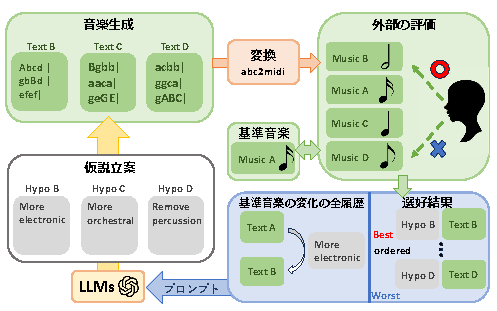
\includegraphics[width=1.0\linewidth]{figs/2/Hidaka_ICPL_arch.pdf}
    \caption{ICPLを作曲AIに応用したシステム構成図（\cite{hidaka_ICPL}より引用）}
    \label{fig:Hidaka_ICPL_arch}
\end{figure}

\begin{figure}[t]
    \centering
    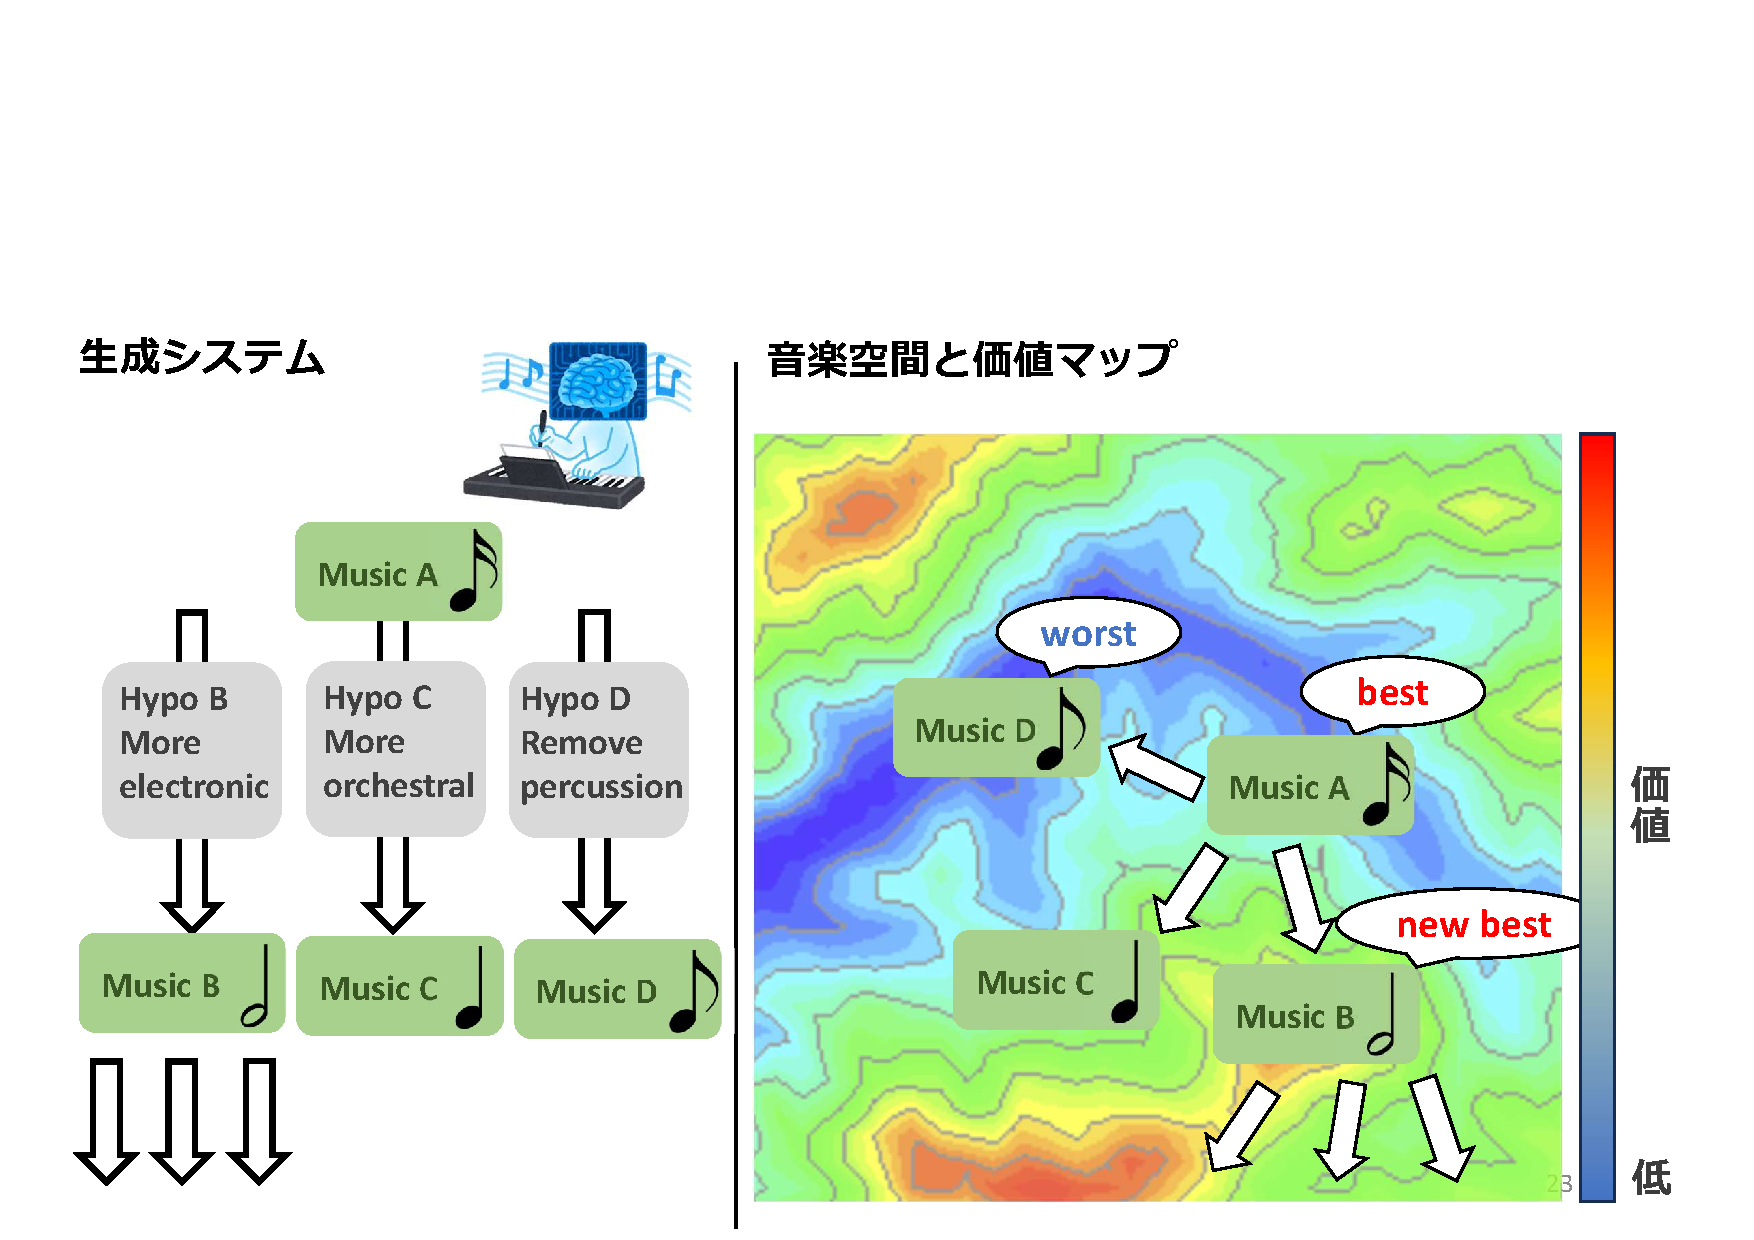
\includegraphics[width=1.0\linewidth]{figs/2/Hidaka_system_image.pdf}
    \caption{ICPLで人の好みを最大化する音楽の探索イメージ（\cite{hidaka_ICPL}より引用）}
    \label{fig:Hidaka_system_image}
\end{figure}

\subsection{AIによる代替と人間の主体性}
\label{subsec:human_creativity}

AIを創造的なパートナーとする際，システムがいかにユーザーの主体性（Agency）を尊重し，創造性を阻害せずに支援できるかは重要な課題である．

\subsubsection{主体性を尊重した最適化支援}
これまでのデザイン支援において，小山らは，ベイズ最適化（Bayesian Optimization）を活用したフレームワーク\cite{BOデザイン提案}を提案している．
従来のデザイン最適化システムでは，システムが生成した案をユーザーに強制的に評価させる（Explicit loop）ものが多く，ユーザーの試行錯誤のプロセスを分断し，主体感を損なう傾向があった．これに対し小山らの手法は，ユーザーがスライダ操作による探索を行っている様子をシステムが「横から観察」し，裏側で非同期的に最適化を行うことで，ユーザーの作業を中断させることなく合理的なデザイン案を提示する．
このアプローチは，ユーザーの自由な探索を阻害しないという点で優れている．しかし，これはあくまでパラメータ空間における数値的な探索支援であり，ユーザーが「どのような意図で」操作しているかという文脈の理解や，言語を通じた相互のコミュニケーションは行われない．すなわち，提示された案を採用するか否かの判断はユーザーに委ねられているものの，そこにはAIとの意味的な対話や共創関係は希薄である．

\subsubsection{LLMとの共創における課題}
一方で，LLMやICPLのような強力な推論・言語能力を持つエージェントとの共創においては，コミュニケーションが可能になる反面，AIが創造プロセスを過度に代替してしまうという新たな課題が生じる．
LLMは膨大な知識量に基づき，対話履歴から高速に最適解らしきものを導き出すことができる（収束的思考）．しかし，Doshiら\cite{人とLLMの共創}による発散的思考と収束的思考に関するランダム化実験では，生成AIがアイデア出しを代替することで，ユーザー自身の思考機会を奪い，かえって創造性を阻害する可能性（Thinking-Halt）が示唆されている．

すなわち，単にユーザーの指示通りに「正解」を出すだけのシステムでは，効率性は向上しても「相互創発的なパートナーシップ」とはなり得ない．AIはユーザーの思考を代替するのではなく，小山らの研究のように主体性を尊重しつつ，多様な選択肢の提示や予期せぬ提案によってユーザーの発散的思考を刺激する役割を担うべきである．
本研究が提案するシステムにおいて，ユーザーによるフィードバックのループ（Human-in-the-loop）を重視し，かつ言語による意図のすり合わせを行うのは，この「主体性の維持」と「意味的な共創」を両立させるためである．


\section{音楽生成における制御と演奏レンダリング}
\label{sec:related_work}

% -----------------------------------------------------------
% 2.1 一般的な生成モデルの話
% -----------------------------------------------------------
\subsection{音楽生成モデルの動向と制御性}
\label{subsec:trends}
近年，深層学習を用いた音楽生成技術は急速に発展している．特に，MusicGen\cite{MusicGen}やMusicLM\cite{MusicLM}などの大規模モデルは，テキストプロンプトから多様なジャンルの楽曲を生成することを可能にした．
しかし，これらのモデルはテキストという抽象的な指示に依存しているため，メロディやリズムといった音楽的な詳細構造（Low-level content）を意図通りに制御することは困難である．Linら\cite{Lin2024}が指摘するように，実用的な音楽制作においては，抽象的なイメージだけでなく，楽譜やMIDIといった具体的な条件付け（Conditioning）に基づく制御が不可欠である．
この課題に対し，近年ではControlNet\cite{ControlNet}やAdapter技術を用い，事前学習済みモデルに追加の制御入力を与える手法が注目されている．

% -----------------------------------------------------------
% 2.2 具体的なタスク（演奏表現）の話
% 最初の画像の論文(2.2 Performance Rendering)の内容を反映
% -----------------------------------------------------------
\subsection{演奏レンダリング (Performance Rendering)}
\label{subsec:performance_rendering}
演奏レンダリングとは，入力された楽譜情報（Score/MIDI）に対し，人間らしい自然な演奏オーディオを生成するタスクである．
これはテキスト読み上げ（TTS）と類似した目的を持つが，音楽特有の多声性（Polyphonic）や，楽譜上の時間と実際の演奏時間の非線形な対応関係（テンポルバート等）により，その難易度は高い．単に楽譜通りの音高・音価を再現するだけでなく，演奏者の解釈による「表現の多様性（Performance Variability）」をいかにモデル化するかが，本タスクにおける重要な課題となっている．

% -----------------------------------------------------------
% 2.3 使用するモデルと数式の話
% -----------------------------------------------------------
\subsection{RenderBoxと基礎理論}
\label{subsec:RenderBox}
本研究では，テキストおよびMIDIによる表現豊かな演奏生成を実現するために，RenderBox\cite{RenderBox}アーキテクチャを採用する．
RenderBoxは，Stable Audio Open\cite{stable-audio-open}を基盤とした潜在拡散モデル（Latent Diffusion Models）であり，そのバックボーンには **DiT (Diffusion Transformer)**\cite{DiT-base} が用いられている．

従来の拡散モデルでは，ノイズ除去ネットワークとしてCNNベースのU-Net\cite{UNet}が標準的に利用されてきた．しかし，U-Netは局所的な特徴抽出に優れる反面，音楽のような長い時系列データにおける大域的な文脈を捉える能力に課題があった．これに対し，Transformer構造を持つDiTは，Self-Attention機構によりデータ全体の依存関係を効率的に学習可能であり，テキストやMIDIといった異なるモダリティの条件付けを柔軟に統合できる利点がある．

また，モデルの学習においては，生成品質と安定性を向上させるために **$v$-objective**\cite{v-prediction} と呼ばれる定式化を採用している．
これは，拡散過程におけるノイズ $\epsilon$ ではなく，速度 $v$ を予測対象とする手法である．時刻 $t$ における潜在変数を $z_t$，ノイズスケジュールに基づく係数を $\alpha_t, \sigma_t$ とすると，ターゲットとなる $v_t$ および損失関数 $\mathcal{L}$ は以下のように定義される．

\begin{align}
    v_t &\equiv \alpha_t \epsilon - \sigma_t z_0 \\
    \mathcal{L} &= \mathbb{E}_{t, z_0, \epsilon} \left[ \| v_t - \hat{v}_\theta(z_t, t, c) \|^2 \right]
\end{align}

ここで $\hat{v}_\theta$ はモデルの出力，$c$ はテキストやMIDIによる条件入力を表す．この手法を採用することで，特にS/N比が低いタイムステップにおける学習が安定し，演奏表現の微細なニュアンスの再現が可能となる．

\begin{figure}[h]
    \centering
    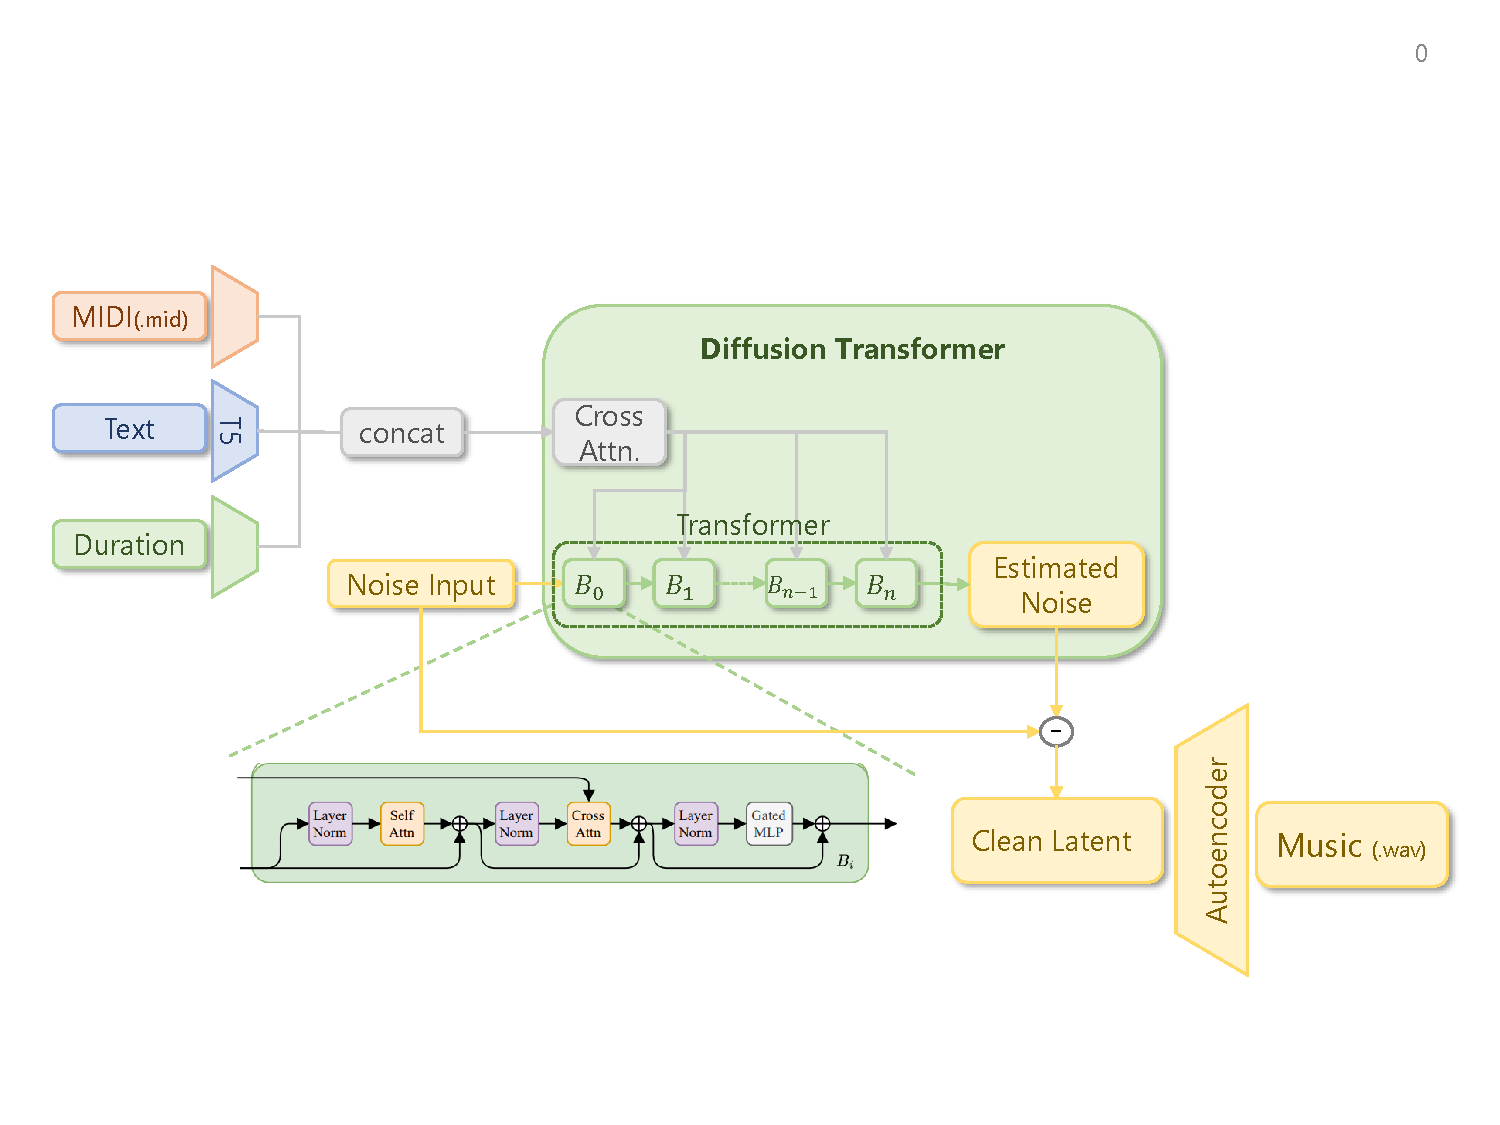
\includegraphics[width=1.0\linewidth]{figs/2/RenderBox_arch.pdf}
    \caption{RenderBoxのアーキテクチャ概要}
    \label{fig:RenderBox_arch}
\end{figure} %理論
\chapter{提案手法}
\label{chap:提案手法}

本章では，ユーザーとAIが対等なパートナーとして音楽表現を共創するためのシステム構成，およびその具体的な処理手順について述べる．提案システムは，人間とAIが交互に演奏プランを提示し合うループ構造を基盤とし，言語モデルによる高度な意図解釈機能を組み込んでいる．

\section{システム概要}
\label{sec:システム概要}

提案システムの全体構成を図\ref{fig:proposed_system}に示す．
本システムは，既存の共創フレームワークであるICPLを拡張したものである．従来のICPLでは，ユーザーはAIが提示した候補についてランキング評価を行っていたが，本手法では自然言語によるフィードバック（コメント機能）を導入した．これにより，ユーザーは単なる「選択」だけでなく，「もう少し優しく」「テンポを揺らして」といった具体的な意図をエージェントに伝達することが可能となる．

\begin{figure}[h]
    \centering
    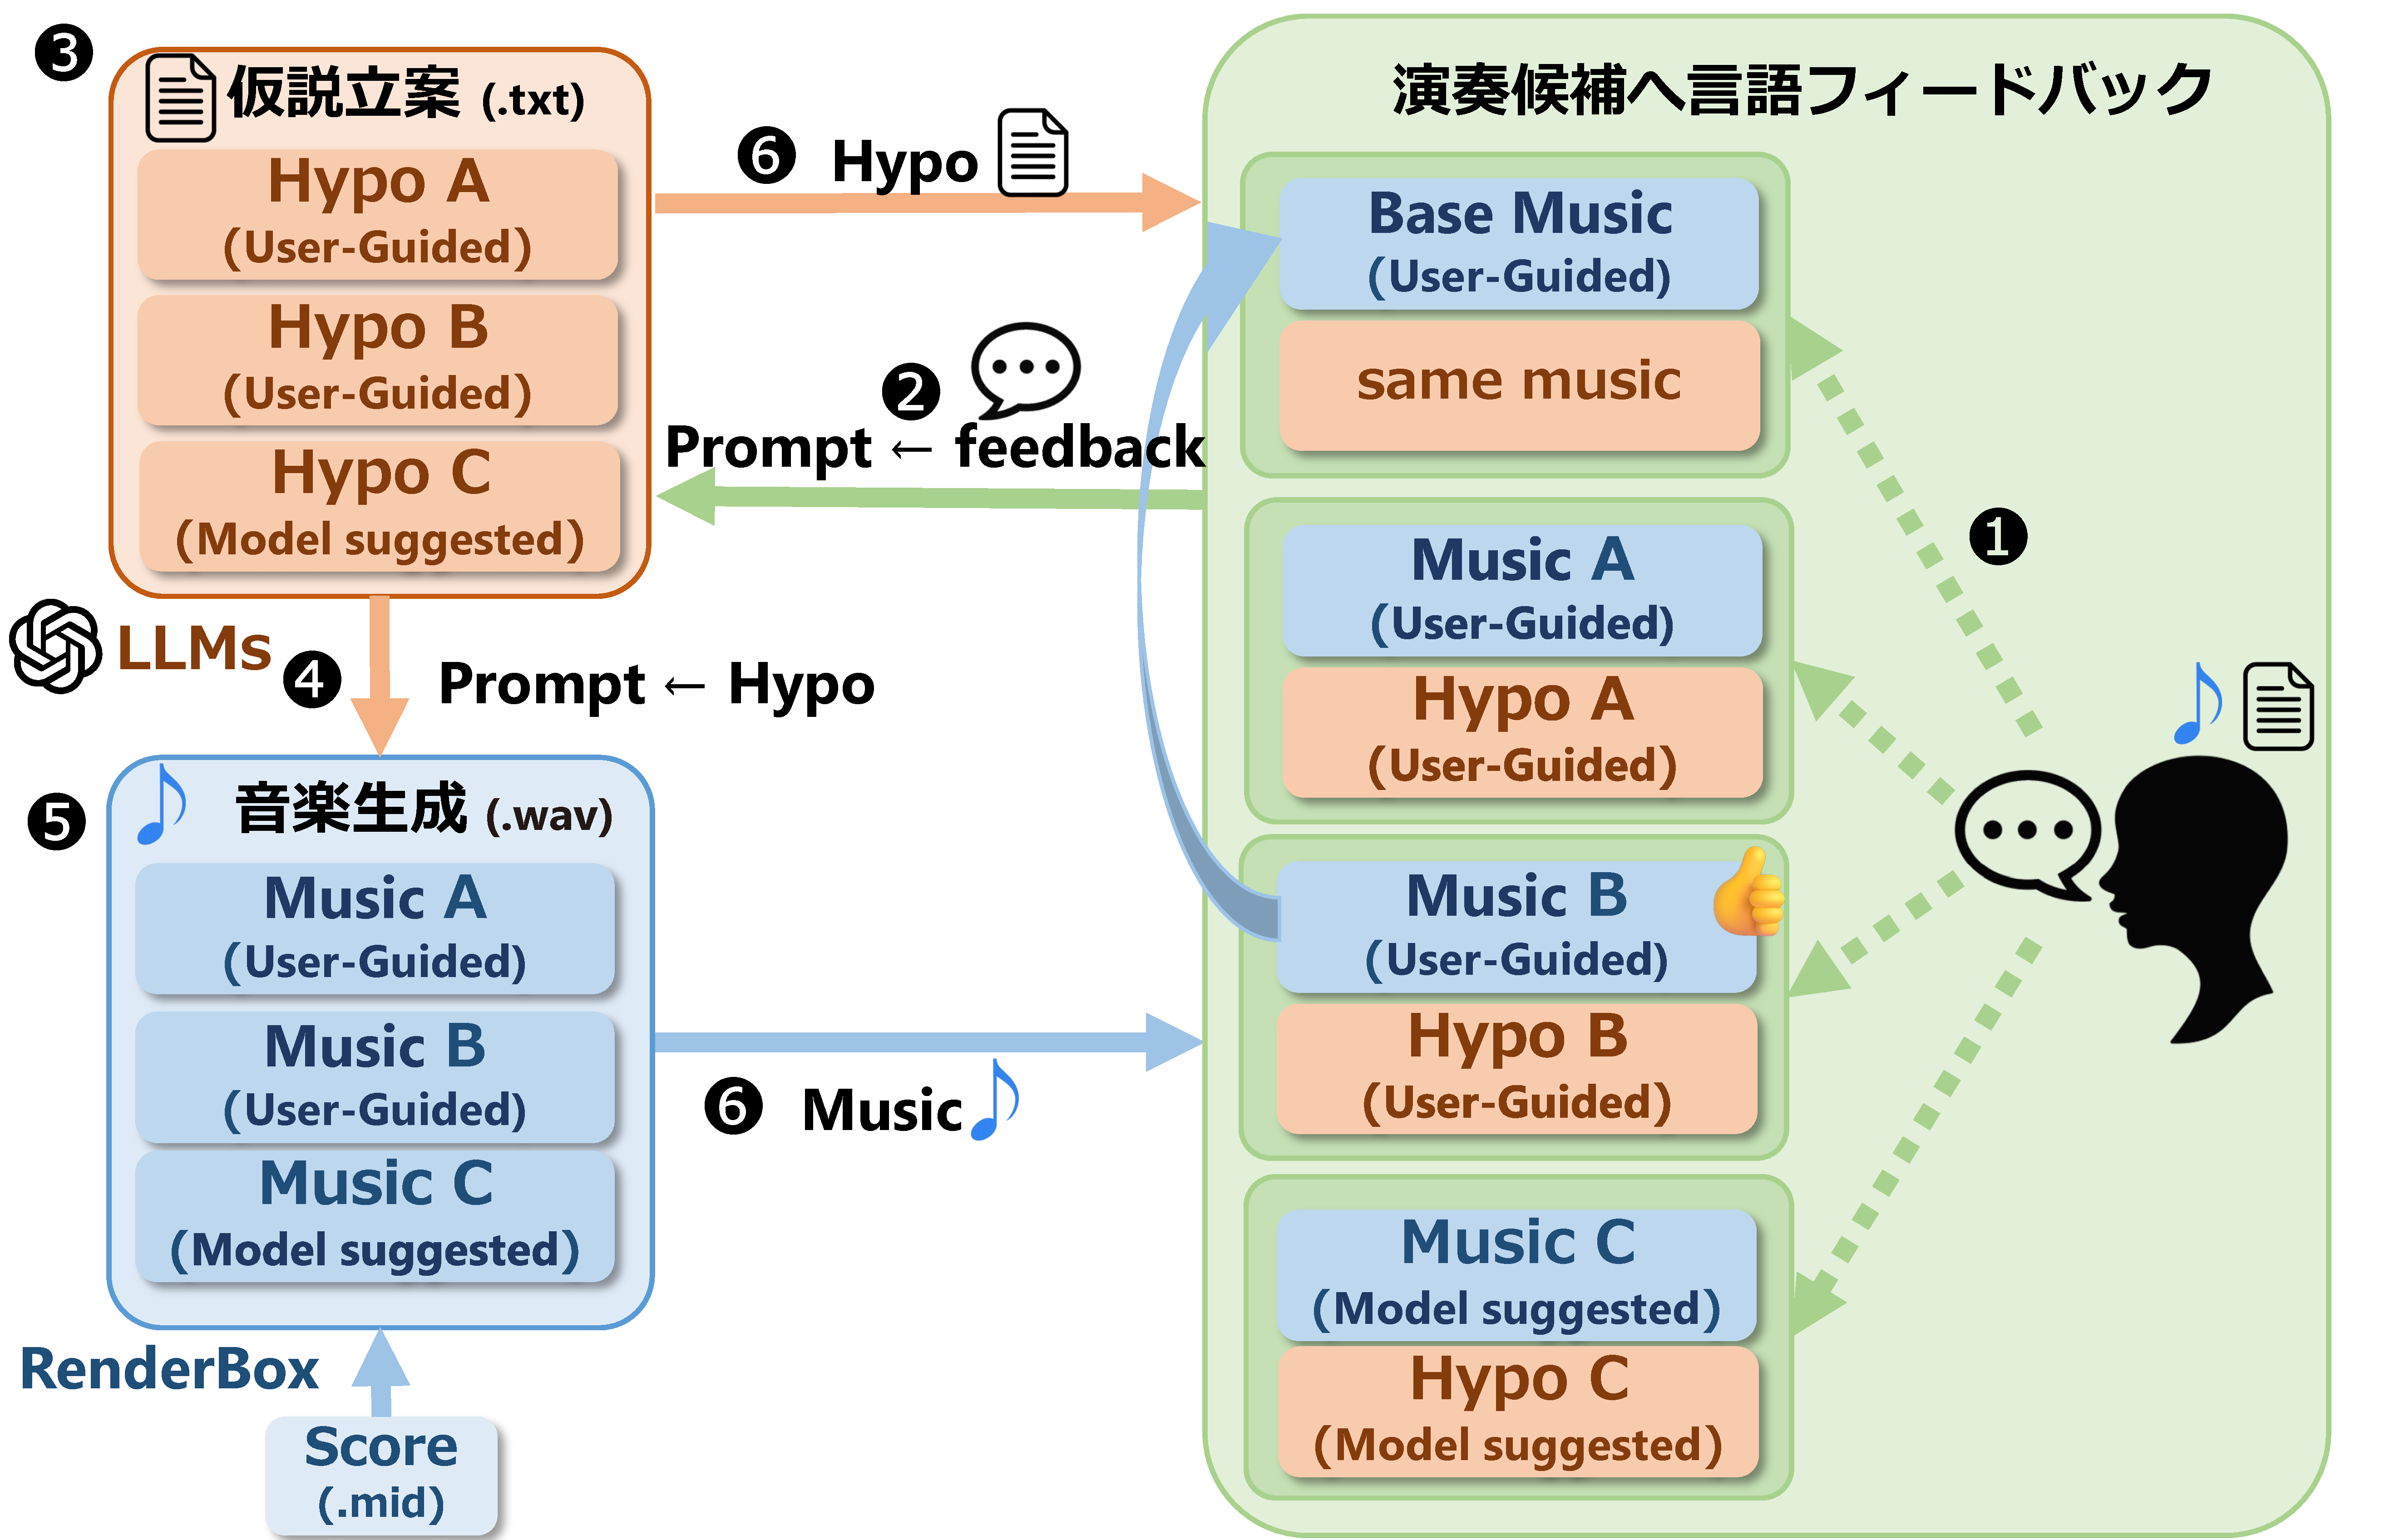
\includegraphics[width=1.0\linewidth]{figs/3/proposed_system.pdf}
    \caption{提案システム構成図}
    \label{fig:proposed_system}
\end{figure}

\section{対話システムとアルゴリズム}
\label{sec:対話システム}

本システムの核となる対話エージェント（Movot Agent）の推論エンジンには，OpenAIの \textbf{GPT-5} (reasoning\_effort=low) を採用した．このモデルは，ユーザーの抽象的な感性語を具体的な演奏パラメータ（強弱，速度，アーティキュレーションなど）へ変換する役割を担う．

システム全体の処理フローをアルゴリズム\ref{alg:overall}に，エージェント内部で行われる意図解釈と演奏生成の詳細プロセスをアルゴリズム\ref{alg:agent}に示す．

\begin{algorithm}
\caption{提案システムの全体処理アルゴリズム}
\label{alg:overall}
\begin{algorithmic}[1]
\Require Participant ID $ID$, Experiment Order $O \in \{Manual \to AI, AI \to Manual\}$

\State \textbf{Initialize:}
\State Load metadata $M$ (Title, Composer, Instrument) from database.
\State Analyze historical context $C_{hist}$ using LLM via \textit{analyze\_song.txt}.
\State Extract professional performance features $C_{perf}$ via \textit{MidiCaps} summary.
\State Generate initial synthesis $A_0$ with neutral prompt.

\State \textbf{Section 1 (Manual Prompting):}
\While{$step < Manual\_Target$}
    \State Receive user expression $E$ and speed index $S$.
    \State $P \gets$ Construct text prompt using $E$ and $SPEED\_TIERS[S]$.
    \State $D \gets$ Calculate duration based on $SPEED\_FACTORS[S]$.
    \State $A_{step} \gets$ AudioGeneration($P, MIDI, D$).
\EndWhile

\State \textbf{Section 2 (AI Co-Creation with Movot Agent):}
\State Initialize Agent with $C_{hist}$, $C_{perf}$, and $A_0$.
\While{$step < AI\_Target$}
    \State Execute \textbf{Algorithm 2} to generate three hypotheses.
    \State Present candidates $\{H_A, H_B, H_C\}$ to user.
    \State $Winner \gets$ User selection; Store feedback for next loop.
\EndWhile
\end{algorithmic}
\end{algorithm}

\begin{algorithm}
\caption{AIエージェントによる意図解釈と演奏生成のアルゴリズム}
\label{alg:agent}
\begin{algorithmic}[1]
\Require User Feedback $f_t$, Musical Context $M_1$ (Static), Interaction History $M_2$ (Dynamic)

\State \textbf{Holistic Feedback Analysis:}
\State $S_{curr} \gets$ Detect speed tag from the previous winner's prompt.
\If{$f_t$ requests speed change}
    \State Apply \textbf{AGGRESSIVE Speed Logic}: Shift speed category by 2 steps in $SPEED\_SCALE$.
\EndIf

\State \textbf{Hypothesis Generation (LLM Reasoning):}
\State \textbf{Strategy A (Direct):} Map $f_t$ strictly to musical articulation.
\State \textbf{Strategy B (Variation):} Propose alternative touch/style based on $f_t$.
\State \textbf{Strategy C (Contextual):} Blend $f_t$ with $C_{hist}$ and $C_{perf}$ from $M_1$.
\State \textbf{Constraint Check:} Ensure $H_A$ and $H_B$ use contrasting articulation (e.g., Legato vs. Rhythmic).

\State \textbf{Parallel Audio Synthesis:}
\For{each $H_i \in \{H_A, H_B, H_C\}$}
    \State $P_i \gets$ ``Expressive Performance, [Instrument], $H_i.keywords$''
    \State $D_i \gets$ Calculate duration for $H_i.speed\_tag$.
    \State $A_{i,t} \gets$ DiffusionModel($P_i, D_i, MIDI$).
\EndFor
\State \textbf{Output:} Reasoning logs and Audio candidates $\{A_A, A_B, A_C\}$.
\end{algorithmic}
\end{algorithm}



\begin{table}[htbp]
\centering
\caption{時系列順のLLMプロンプト構成とRoleの定義}
\label{tab:prompt_flow}
% \textwidth で「ページ幅いっぱい」を指定
% 最後の列を 'X' にすると、残りのスペースに合わせて自動改行されます
\begin{tabularx}{\textwidth}{l c l l} 
\hline
\textbf{フェーズ} & \textbf{Role} & \textbf{タイミング} & \textbf{提供される情報} \\ \hline
1. 楽曲分析 & System & 初期化時 & エージェントの役割 \\
 & & & 楽曲のタイトル \\
 & & & 作曲家名 \\ \hline
2. 状況設定 & System & 共創開始 & Movotの人格 \\
 & & & RenderBoxの能力 \\
 & & & プロ演奏のデータ \\ \hline
3. 対話ループ & User & 毎ループ実行 & 選択された演奏案 \\
 & & & フィードバック内容 \\
 & & & 過去の対話履歴 \\ \hline
4. 制約の適用 & User/System & 毎ループ実行 & 速度調整ルール \\
 & & & 提案間の差別化戦略 \\ \hline
\end{tabularx}
\end{table}



\section{UIの構築}
\label{sec:UIの構築}
PythonのGradioライブラリを用いて図？？のようなUIを作成した． %提案手法
\chapter{実験}
\label{chap:実験}

本章では，提案システムの基盤となる音楽生成モデルRenderBoxの訓練詳細，および提案システムの有効性を検証するために実施した被験者実験について述べる．

\section{RenderBoxの訓練}
\label{sec:RenderBoxの訓練}

\subsection{データセット}
RenderBoxの訓練には，ASAP\cite{asap-dataset}，MusicNet\cite{musicnet-dataset}，GAPS\cite{gaps-dataset}，BachViolin\cite{bach-violine-dataset}，ATEPP\cite{atepp-dataset}，ConEspressione\cite{conespressione-dataset}，Vienna4x22\cite{vienna4x22}を使用した．
各データセットは，訓練用データと推論（評価）用データに9対1の割合でランダムに分割して使用した．
各ステージにおけるデータセットの割り当てを表\ref{tab:datasets}に示す．

\begin{table}[htbp]
\centering
\caption{カリキュラム学習の各ステージで使用したデータセット\cite{RenderBox}}
\label{tab:datasets}
\resizebox{\textwidth}{!}{%
\begin{tabular}{llllll}
\hline
\toprule
\textbf{Datasets by stage} & \textbf{Input MIDI} & \textbf{Target Audio} & \textbf{Inst.} & \textbf{Controls / Prompts} & \textbf{Repertoire / Notes} \\ \midrule
\hline
% ▼▼▼ ここを {7} から {6} に修正しました ▼▼▼
\multicolumn{6}{l}{\textit{Stage 0: Synthesis}} \\
ASAP & Score \& & Synth. Score \&  & Piano & - & Common Practice Period \\
 & Performance & Perf. Audio & & & solo piano works \\
MusicNet & Score \& & Synth. Score \&  & Orchestral & - & Classical music with a large \\
 & Performance & Perf. Audio & & & portion of chamber works \\
GAPS & Score & Synth. Score & Guitar & - & Noted classical guitar works \\ \midrule
\hline
% ▼▼▼ ここを {7} から {6} に修正しました ▼▼▼
\multicolumn{6}{l}{\textit{Stage 1: Speed-controlled synthesis}} \\
ASAP & Score & Synth. Score  & Piano & Tempo & Time-varied score synthesis \\
GAPS & Score & Synth. Score & Guitar & Tempo & Time-varied score synthesis \\
MusicNet & Score & Synth. Score & Orchestral & Tempo & Time-varied score synthesis \\ \midrule
\hline
% ▼▼▼ ここを {7} から {6} に修正しました ▼▼▼
\multicolumn{6}{l}{\textit{Stage 2: Expressive Performance}} \\
ASAP & Score & Perf. Audio & Piano & Expressive & Aligned perf. segments \\
GAPS & Score & Perf. Audio & Guitar & Expressive & Aligned perf. segments \\
MusicNet & Score & Perf. Audio & Orchestral & Expressive & Aligned perf. segments \\
BachViolin & Score & Perf. Audio & Violin & Expressive & Bach violin sonata \\ \midrule
\hline
% ▼▼▼ ここを {7} から {6} に修正しました ▼▼▼
\multicolumn{6}{l}{\textit{Stage 4: Style-directioned Performance}} \\
ATEPP-subset & Score & Perf. Audio & Piano & Performer labels & Standard piano repertoire \\
 & & & & &  played by 40+ pianists \\
Con Espressione & Score & Perf. Audio & Piano & Human-annotated & 45 perf. of 9 excerpts annot. \\
 & & & & expression labels & by 179 participants \\
Vienna 4x22 & Score & Perf. Audio & Piano & Performer labels & 4 short pieces played by 22 \\
 & & & & & pianists each \\ \bottomrule
 \hline
\end{tabular}%
}
\end{table}

\subsection{カリキュラム学習}
\label{subsec:カリキュラム学習}

本研究では，RenderBoxの学習においてカリキュラム学習を採用した．学習は段階的にタスクの難易度や条件を変更しながら進められる．
元のRenderBoxの論文では，意図的に演奏ミスを含ませてモデルのロバスト性を向上させるStage 3が存在するが，本研究では「理想的な表現生成」に焦点を当てるため，このStage 3は省略し，Stage 0, 1, 2, 4の順で学習を行った．

学習環境として，GPUにはNVIDIA A100 (80GB)を2〜3枚使用した．学習時のハイパーパラメータについては，バッチサイズを108〜112に設定し，計算資源の効率的な利用を図った．

\subsection{性能評価指標}
\label{subsec:性能評価指標}

本研究では，生成された演奏の品質，楽曲の整合性，およびテキスト指示への追従性を評価するために，Evansら\cite{stable-audio-open}によって確立され，stable-audio-metricsに実装されている指標を採用した．具体的には以下の指標を用いる．

\begin{itemize}
    \item \textbf{FAD (Fréchet Audio Distance):}
    生成された音声の品質と多様性を評価する指標である．Cramerら\cite{FAD}によるOpenL3埋め込み表現を用いて，生成音声の分布と正解データ（Ground Truth）の分布間の距離を算出する．なお，本実験におけるFADの算出にあたっては，生成された演奏群と，その楽曲が属するデータセットのテスト用データセット（Ground Truth）との間で比較を行った．
    
    \item \textbf{CLAP Score:}
    テキストプロンプトと生成音声の意味的な整合性を評価する指標である．Wuら\cite{clap}によるLAION-CLAP空間における，入力テキストプロンプトと出力音声の埋め込みベクトル間の距離として計算される．
    
    \item \textbf{Chroma Similarity (Pitch Accuracy):}
    演奏生成タスクにおいては，正しい楽曲（楽譜通りの音高）が演奏されていることが不可欠である．そこで，ピッチ方向の正確性を評価するために，MusicGen-Melody\cite{copet2023}の評価手法に着想を得たChroma類似度を用いる．
    生成音声と正解音声は必ずしも時間的に整合（タイムアラインメント）していないため，まずクロマグラムに対して動的時間伸縮（DTW: Dynamic Time Warping）を適用し，大まかなフレーム対応を推定する．このアライメントに基づき，対応するフレーム間のコサイン類似度を計算する．さらに，アライメントのコスト（DTWコスト）をペナルティ項として組み込み，重み係数 $\lambda = 10^{-3}$ でスケーリングして最終的なスコアとする．
    
    \item \textbf{Tempo Deviation:}
    生成された演奏のテンポが，プロンプトで指定されたテンポ（Table \ref{tab:datasets}参照）の範囲内に収まっているかを評価する．
    \texttt{madmom}ライブラリを用いて生成音声のテンポを推定し，プロンプトによって調整された楽譜上の目標テンポに対する差異（逸脱度）をパーセンテージで算出する．
\end{itemize}

\section{被験者実験}
\label{sec:被験者実験}

提案システムにおける「Human-in-the-Loop」および「LLMによる仮説生成」の有効性を検証するため，被験者実験を行った．

\subsection{被験者実験の概要}
\label{subsec:被験者実験の概要}

被験者は男性4名，女性4名の計8名である．被験者の音楽的背景（楽器経験年数，普段聴く音楽ジャンル等）については，実験後のアンケートにより収集した．被験者の属性詳細を図\ref{fig:participants_demographics}に示す（または後述の表\ref{tab:questionnaire_items}のD項にて収集）．

% 図を入れる場合
% \begin{figure}[htbp]
% \centering
% \includegraphics[width=0.8\textwidth]{figures/demographics.png}
% \caption{被験者の音楽的バックグラウンド}
% \label{fig:participants_demographics}
% \end{figure}

本実験では，システムが提示する演奏に対するフィードバックを通じて，ユーザーが理想とする演奏表現を探索するプロセスを評価対象とする．

\subsection{被験者実験の手順}
\label{subsec:被験者実験の手順}

実験は，共通の導入フェーズである「実験0」を行った後，比較対象となる2つの条件「実験1（手動プロンプト）」と「実験2（LLMプロンプト生成）」を順不同（またはカウンターバランスをとって）実施した．具体的な手順は以下の通りである．

\subsubsection*{実験0：初期ループ（共通）}
まず，システムの使用感に慣れるため，以下の手順で最初の演奏生成を行う．
\begin{enumerate}
    \item ユーザーは課題曲のScoreに基づく機械的な演奏を聴取する．
    \item その曲に対する「理想の感性的な表現」を言語化し，システムに入力する（図\ref{fig:proposed_system}の(1)(2)）．
    \item 入力されたテキストを直接プロンプトとしてRenderBoxに入力し，音楽を生成する（図\ref{fig:proposed_system}の(4)(5)）．
    \item ユーザーは生成された演奏を聴き，フィードバック（コメント）を行う（図\ref{fig:proposed_system}の(6)(1)）．このとき生成された演奏を，以降の実験における「基準演奏」とする．
\end{enumerate}

\subsubsection*{実験1：人が直接プロンプトを入力（ベースライン）}
ユーザー自身が表現を言語化し，試行錯誤する条件である．
\begin{enumerate}
    \item ユーザーは基準演奏に対し，改善したい点や新たなイメージをプロンプトとして直接入力する（図\ref{fig:proposed_system}の(2)）．
    \item 入力されたプロンプトをもとに，RenderBoxが音楽を生成する（図\ref{fig:proposed_system}の(5)）．
    \item ユーザーは生成演奏に対し，フィードバック（コメントと満足度ランキング）を行う（図\ref{fig:proposed_system}の(6)(1)）．
    \item ユーザーが演奏に満足するか，または規定のループ回数上限に達するまで，手順1〜3を繰り返す．
\end{enumerate}

\subsubsection*{実験2：LLMがプロンプトを生成（提案手法）}
LLMがユーザーのフィードバックを解釈し，多様な表現仮説を提案する条件である．
\begin{enumerate}
    \item ユーザーのフィードバック（コメントとランキング）をLLMに入力する（図\ref{fig:proposed_system}の(2)）．
    \item LLMはフィードバックに基づき，以下の3種類の仮説（プロンプト）を立案する（図\ref{fig:proposed_system}の(3)）．
    \begin{itemize}
        \item \textbf{Hypo A, B:} ユーザーのフィードバックに忠実な改善案．
        \item \textbf{Hypo C:} LLMの音楽知識に基づき，今までと異なる表現解釈や意外性を含んだ提案（Deviated hypothesis）．
    \end{itemize}
    \item 3つの仮説をRenderBoxに入力し，3種類の候補演奏を生成する（図\ref{fig:proposed_system}の(4)(5)）．
    \item ユーザーは3つの候補演奏および基準演奏を聴き比べ，フィードバックを行うとともに，最も好ましい演奏を選択する．選択された演奏は次のループの「基準演奏」となる（図\ref{fig:proposed_system}の(6)(1)）．
    \item ユーザーが満足するか，ループ上限回数に達するまで繰り返す．
\end{enumerate}

\subsection{評価指標}
\label{subsec:評価指標}

実験結果の分析には，以下の観点および指標を用いる．

\subsubsection*{相互創発性 (Co-creativity)}
エージェント（AI）からの提案が，ユーザーの意図を超えて新しい価値を生み出したかを評価する．
\begin{itemize}
    \item \textbf{客観的評価:} 実験2において，LLMが独自の解釈を加えた「Music C（Hypo Cに基づく演奏）」が，次のループの基準演奏としてユーザーに選択された回数や割合．
    \item \textbf{主観的評価:} 「Music C」の演奏やその解釈テキストに対し，ユーザーが「意外だが良い」「新しい発見があった」と感じたかをアンケート（Q7, Q8）により評価する．
\end{itemize}

\subsubsection*{ユーザビリティ (Usability)}
システムが効率的かつ意図通りに機能したかを評価する．
\begin{itemize}
    \item \textbf{客観的評価:} ユーザーが最終的な満足に至るまでに要したループ回数を比較する．実験1より実験2の方が少ない回数で満足した場合，効率が良いと判断する．
    \item \textbf{主観的評価:} 「意図通りの演奏が生成されたか」「プロンプト生成の手間が軽減されたか」といった点をアンケート（Q4, Q6）により評価する．
\end{itemize}

実験に使用したアンケート項目の一覧を表\ref{tab:questionnaire_items}に示す．

\begin{table}[htbp]
\centering
\caption{被験者実験で使用したアンケート項目一覧}
\label{tab:questionnaire_items}
\resizebox{\textwidth}{!}{%
\begin{tabular}{llp{7cm}l}
\toprule
\textbf{Category} & \textbf{ID} & \textbf{Question Item} & \textbf{Scale} \\ \hline
\midrule
% --- 属性 ---
\multirow{4}{*}{Demographics} 
 & D1 & 年齢・性別 & Open \\
 & D2 & 普段音楽を聴く頻度・ジャンル & Open \\
 & D3 & 楽器演奏経験の有無とその年数 & Open \\
 & D4 & （事務用）被験者ID・名前 & - \\ \hline
\midrule
% --- 全体評価 ---
\multirow{4}{*}{\shortstack{Overall\\Satisfaction}} 
 & Q1 & セクション1（手動）で生成された演奏に満足しましたか？ & 5-point Likert \\
 & Q2 & セクション2（対話）で生成された演奏に満足しましたか？ & 5-point Likert \\
 & Q3 & どちらのセクションの演奏により満足しましたか？ & 2-AFC \\
 & Q4 & どちらのシステムが使いやすかったですか？ & 2-AFC \\ \hline
\midrule
% --- システム評価 ---
\multirow{2}{*}{\shortstack{System\\Capability}} 
 & Q5 & エージェントはあなたの理想の演奏を正しく推測していましたか？ & 5-point Likert \\
 & Q6 & あなたの指示通りに演奏が変化していましたか？ & 5-point Likert \\ 
\midrule \hline
% --- 相互創発性 (ここが重要) ---
\multirow{4}{*}{\shortstack{Co-creativity\\\& Interaction}} 
 & Q7 & エージェントの提案に，意図と異なりつつも「良い」と思えるものはありましたか？ & 5-point Likert \\
 & Q8 & 対話を通じて，当初イメージしていた曲の目標や雰囲気が変化しましたか？ & 5-point Likert \\
 & Q9 & エージェントとの対話に関する感想・気づき & Free Text \\
 & Q10 & 実験全体の感想 & Free Text \\ \hline
\bottomrule
\end{tabular}%
}
\vspace{1ex}
\small \\
Note: 5-point Likert (1: Strongly Disagree -- 5: Strongly Agree), 2-AFC (2-Alternative Forced Choice)
\end{table} %実験
\chapter{結果}
\label{chap:結果}

\section{RenderBoxの評価}
\label{sec:RenderBoxの評価}

\begin{table}[htbp]
\centering
\caption{RenderBox \cite{RenderBox} との性能比較（括弧内は文献値）}
\label{tab:renderbox_evaluation}
\resizebox{\textwidth}{!}{%
\begin{tabular}{lcccc} % {lcccc{6cm}} から {lcccc} に修正（5列）
\toprule
\textbf{Model} & \textbf{FAD} $\downarrow$ & \textbf{Pitch} $\uparrow$ & \textbf{Tempo} $\downarrow$ & \textbf{CLAP} $\uparrow$ \\ 
\midrule
% --- Stage 0 (w/o align) ---
Stage 0 & 61.8793 & 0.792 & 16.89 & 0.071 \\
 & (839.3) & (0.794) & (0.038) & (0.174) \\ 
\midrule
% --- Stage 2 ---
Stage 2 & 96.2042 & 0.8130 & 18.55 & 0.069 \\
 & (562.58) & (0.753) & (10.39) & (0.265) \\ 
\midrule
% --- Stage 4 ---
Stage 4 & 74.7507 & 0.8093 & 16.00 & 0.068 \\
 & (340.77) & (0.748) & (19.51) & (0.234) \\ % 末尾の余計な & を削除
\bottomrule
\end{tabular}
}
\end{table}

\begin{figure}[htbp]
    \centering
    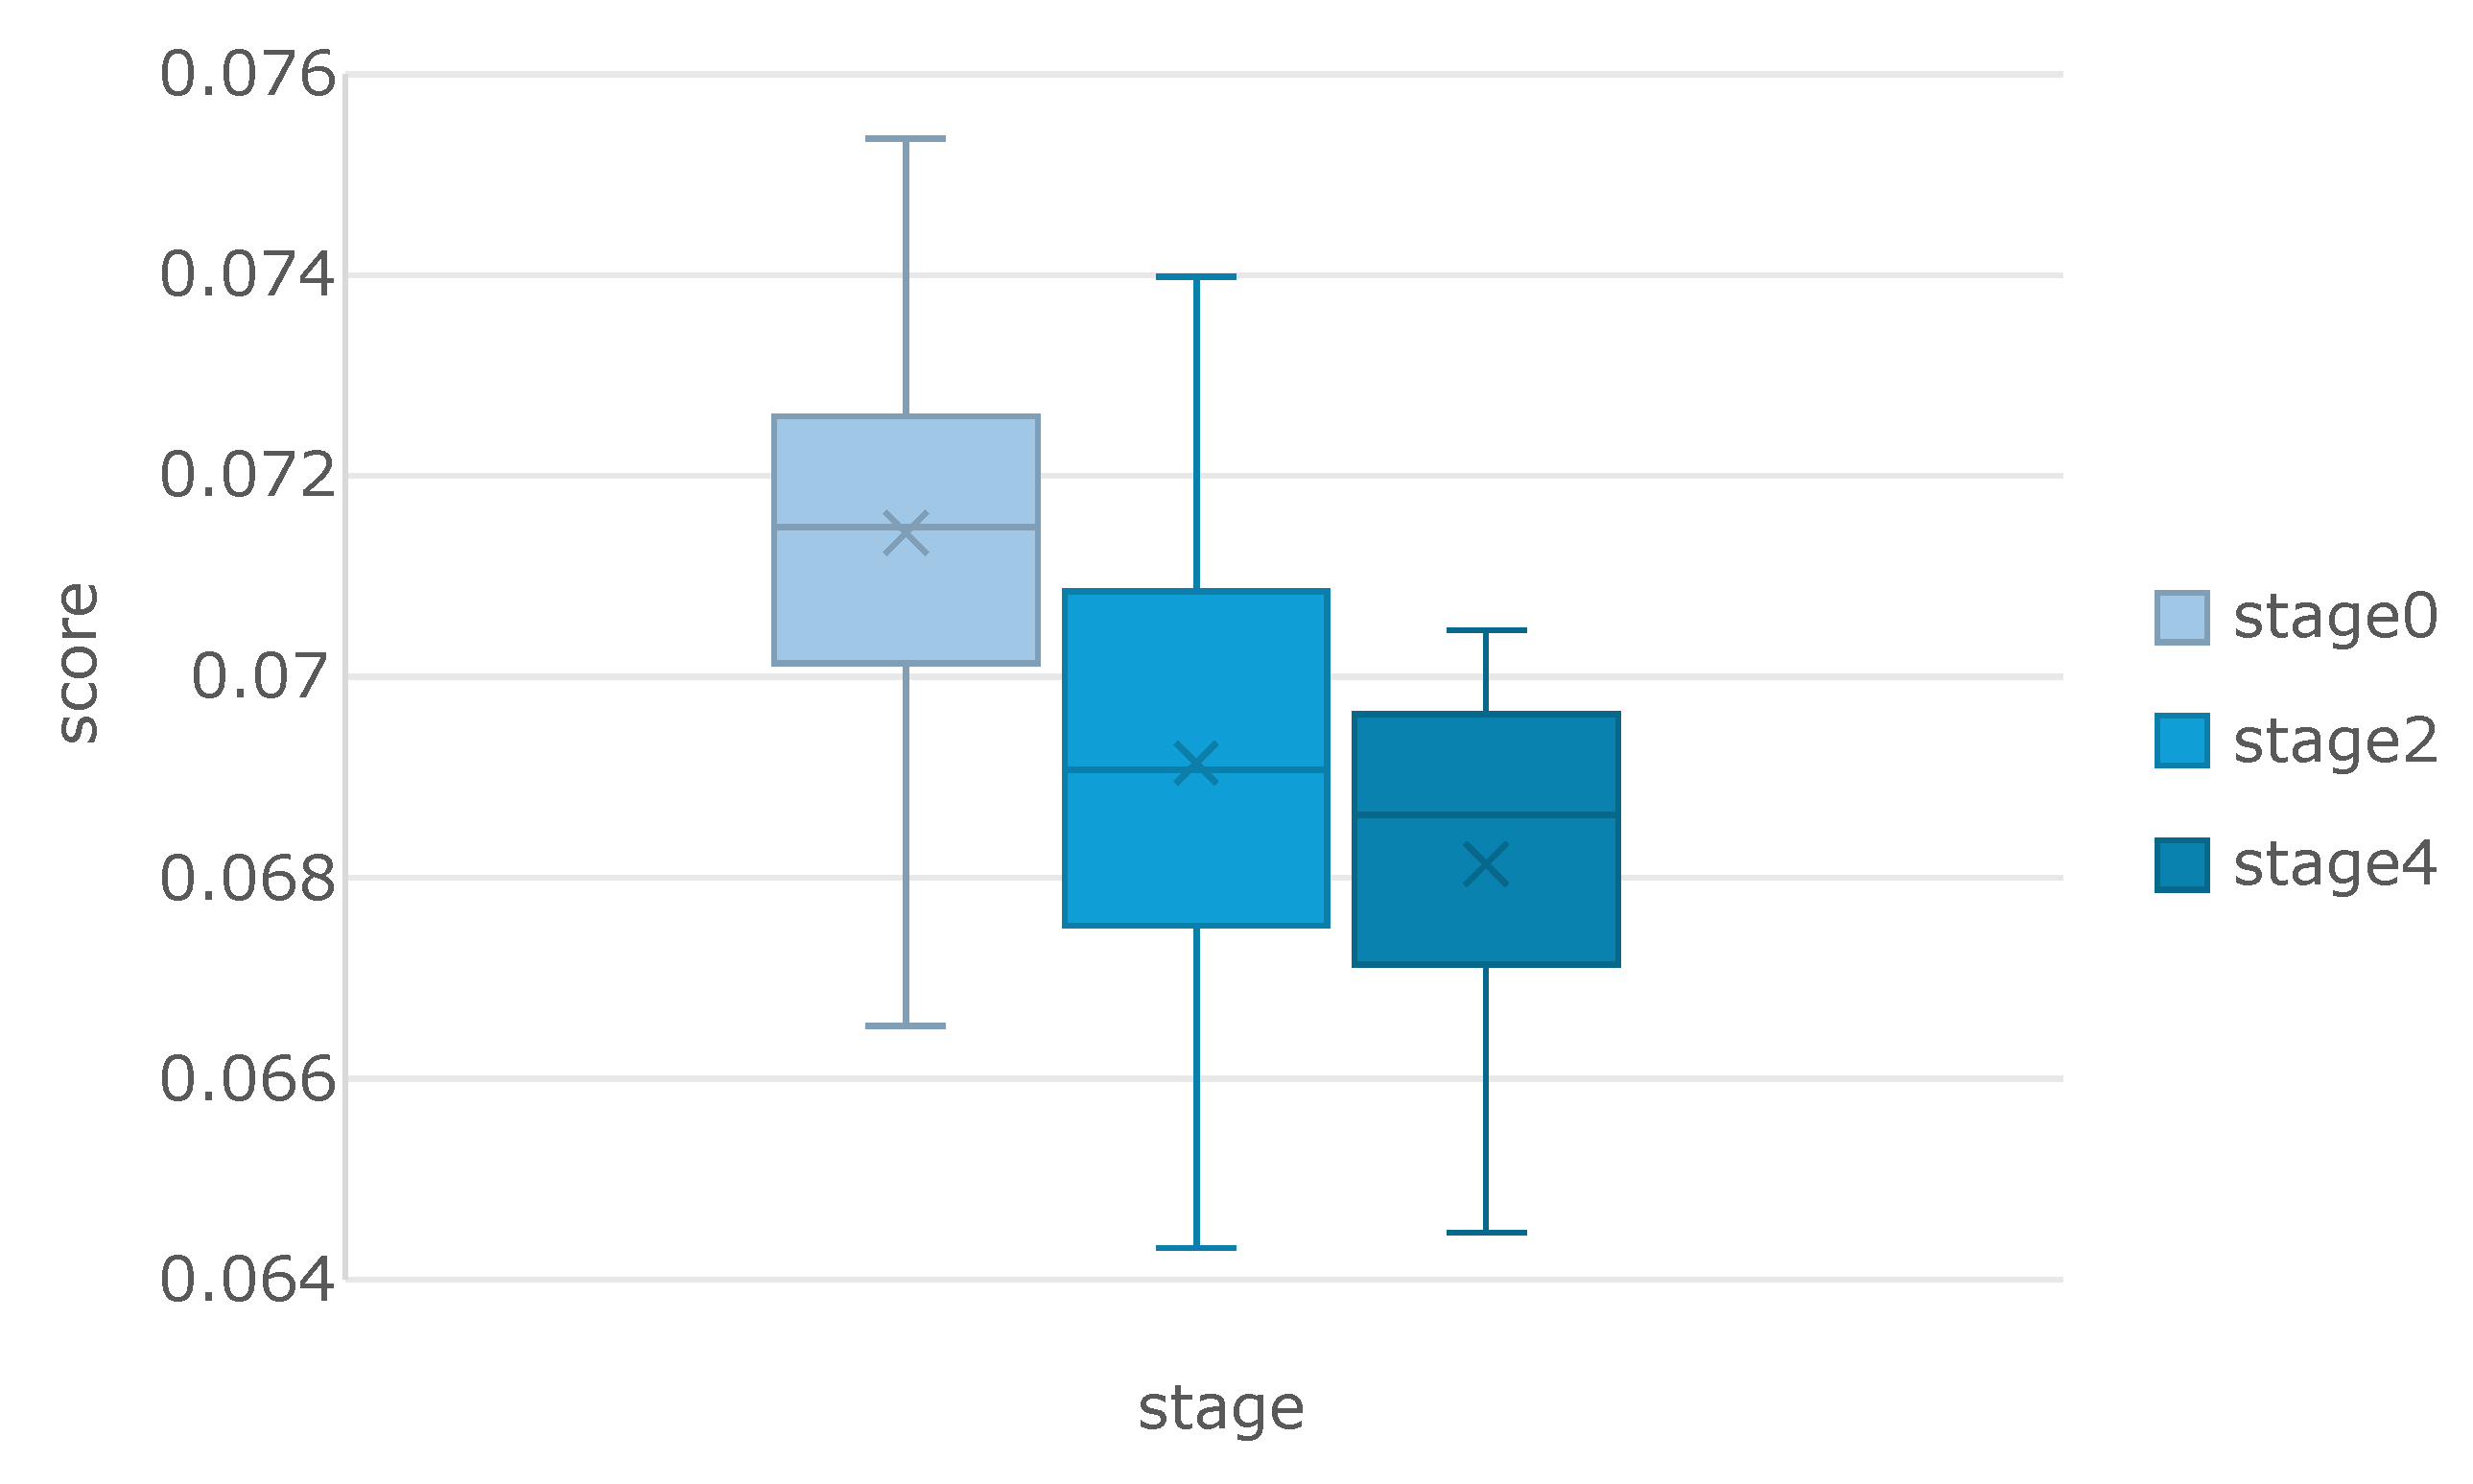
\includegraphics[width=1.0\linewidth]{figs/5/clap.pdf}
    \caption{RenderBoxの性能評価：CLAP score}
    \label{fig:RenderBox_CLAP}
\end{figure}

\begin{figure}[htbp]
    \centering
    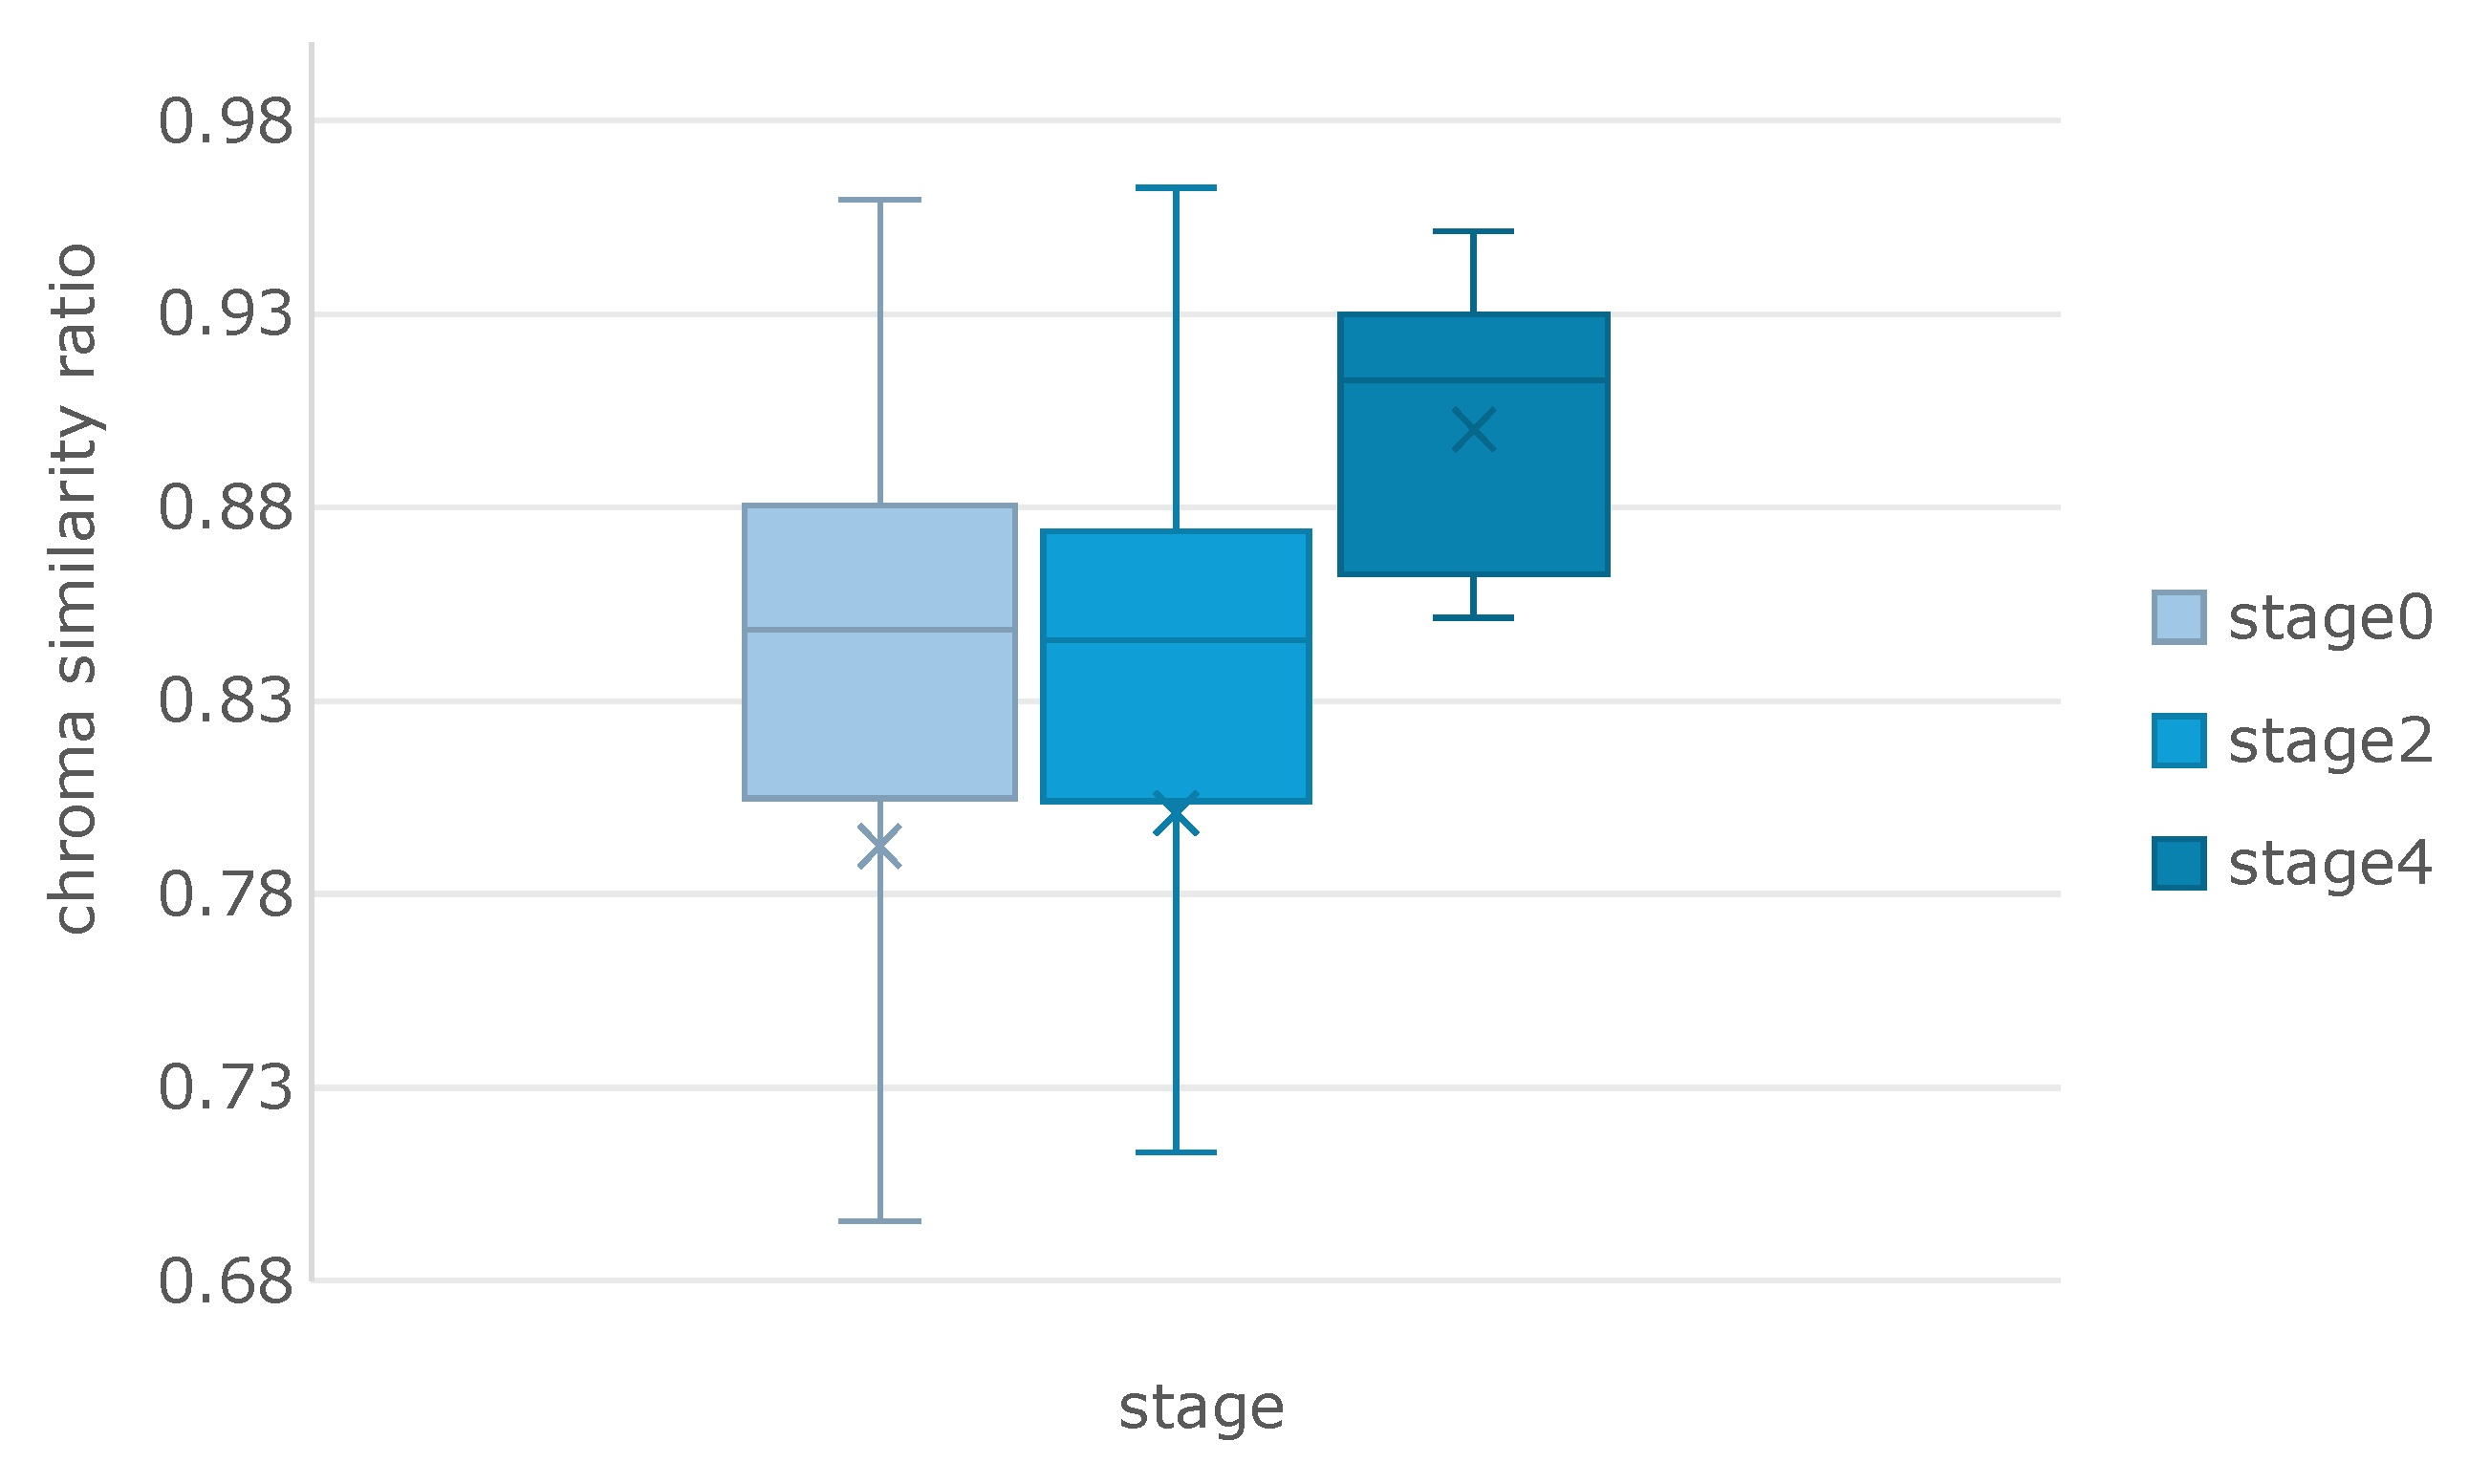
\includegraphics[width=1.0\linewidth]{figs/5/Pitch.pdf}
    \caption{RenderBoxの性能評価：pitchの正確さ}
    \label{fig:RenderBox_pitch}
\end{figure}

\begin{figure}[htbp]
    \centering
    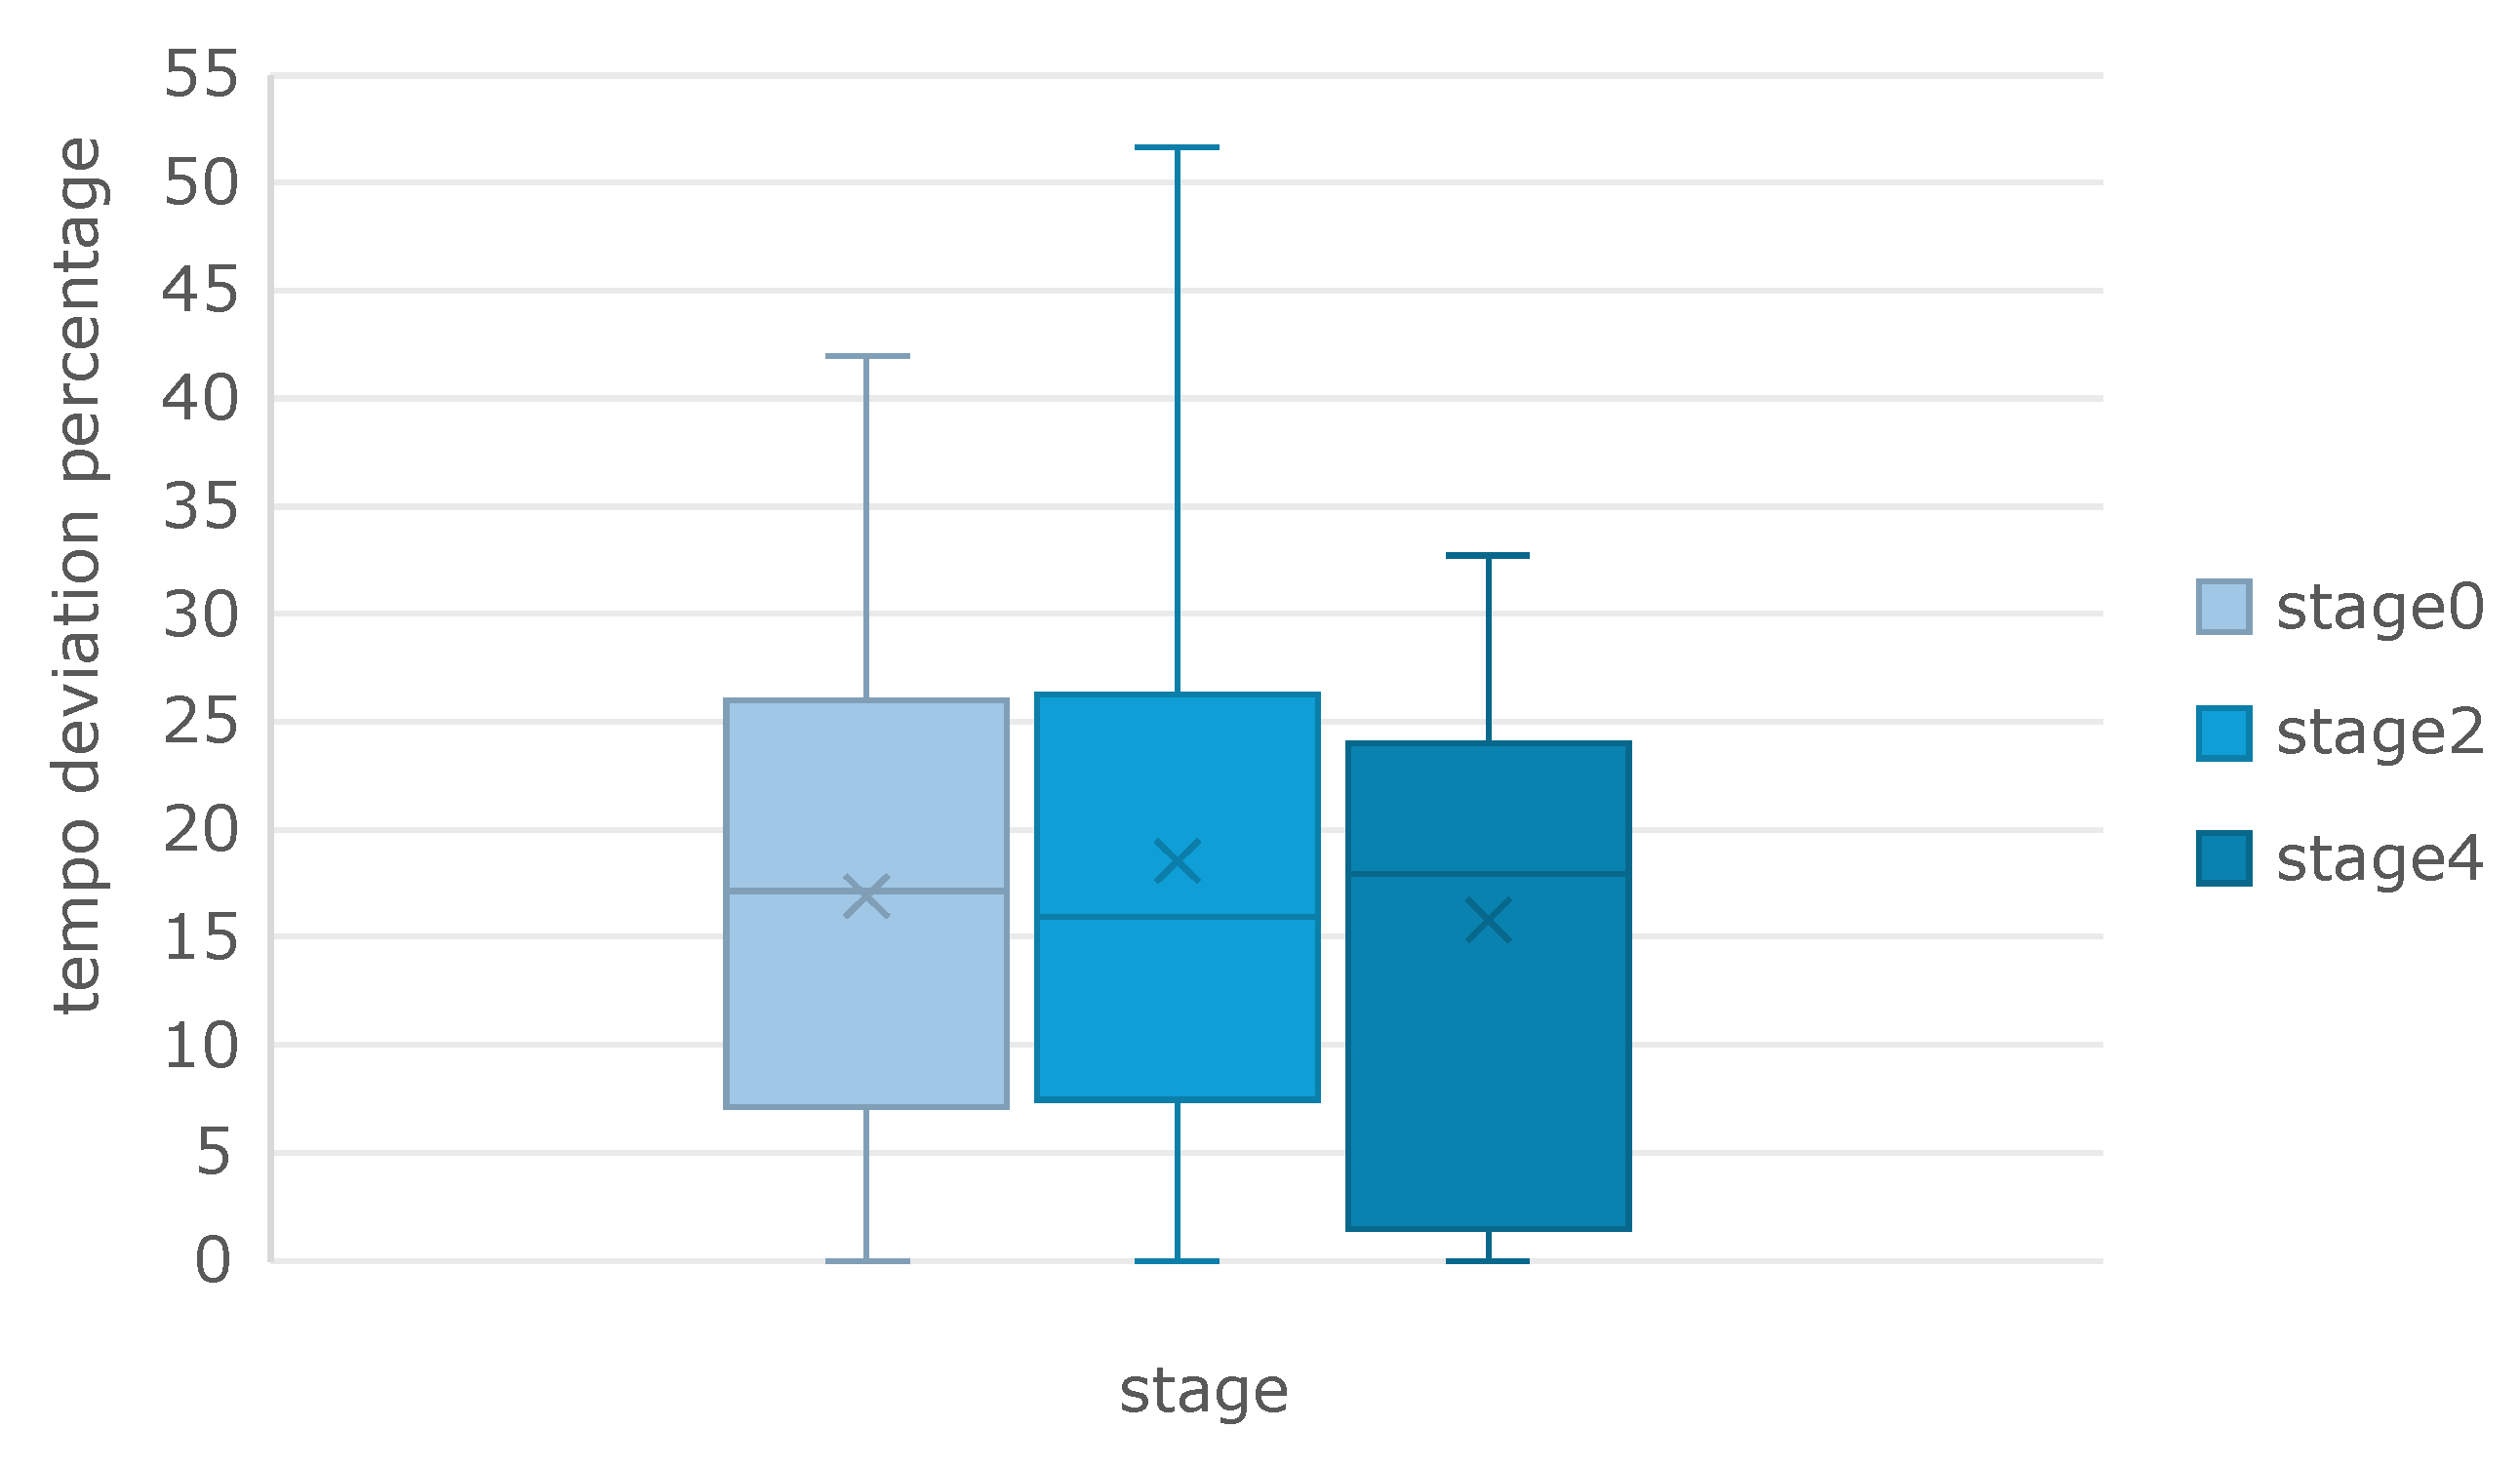
\includegraphics[width=1.0\linewidth]{figs/5/tempo_deviation.pdf}
    \caption{RenderBoxの性能評価：tempoのずれ} % temo -> tempo に修正
    \label{fig:RenderBox_tempo}
\end{figure}

\section{提案システムの評価}
\label{sec:提案システムの評価}

\subsection{客観評価}
\label{subsec:客観評価}
% ここに本文を記述

\subsection{主観評価}
\label{subsec:主観評価}
% ここに本文を記述 %実験
\chapter{考察}
\label{chap:考察}

\section{RenderBoxの性能について}
\label{sec:RenderBoxの性能について}


\section{提案手法について}
\label{sec:提案手法について}


 %考察/議論
\chapter{結論}
\label{chap:結論}
 %結論
\chapter*{謝辞}
\addcontentsline{toc}{chapter}{謝辞}

本研究を進めるにあたり，多大なる助言，ご指導をいただきました，吉川雄一郎教授，堀井隆斗准教授に深く感謝いたします．
 %謝辞
% \input{src/bibliography.tex} %参考文献(直接記述する場合)
\newpage
\addcontentsline{toc}{chapter}{\bibname}
\bibliographystyle{junsrt}
\bibliography{src/references.bib} %参考文献(bibtexを使う場合)
% \newpage
\renewcommand{\bibname}{発表実績}
\addcontentsline{toc}{chapter}{\bibname}
\begin{thebibliography}{99}
% 国際学会(ポスター発表　査読あり)
% 国内学会・シンポジウム等における発表 (すべて査読なし)


% \newpage
% {\Large \bf{本人発表以外の関連発表}}
% \bibitem{}xxx
\end{thebibliography}


 %発表実績(直接記述する場合)
% \input{src/awards.tex} %受賞歴
\input{src/8appendix.tex}
\end{document}